% ============================================================================
% ACE Agent 学习指南 — 面向Python初学者的完整源码解析文档
% 编译方式: xelatex -shell-escape ACE_Agent_Learning_Guide.tex
% 环境要求: TeX Live 2023+ 或 Overleaf (XeLaTeX 编译器)
% ============================================================================
\documentclass[11pt,a4paper]{ctexbook}

% ---------- 页面布局 ----------
\usepackage[a4paper,margin=2.2cm,bottom=2.5cm,headheight=14pt]{geometry}
\usepackage{setspace}
\onehalfspacing

% ---------- 图表与颜色 ----------
\usepackage{graphicx}
\usepackage{float}
\usepackage{booktabs}
\usepackage{longtable}
\usepackage{tikz}
\usetikzlibrary{arrows.meta, positioning, shapes.geometric, shapes.multipart, calc, fit, backgrounds, decorations.pathreplacing}
\usepackage{xcolor}
\usepackage{tcolorbox}
\tcbuselibrary{skins, breakable, listings}

% ---------- 代码展示 ----------
\usepackage{minted}
\setminted[python]{
    fontsize=\footnotesize,
    breaklines=true,
    frame=single,
    numbers=left,
    numbersep=5pt,
    baselinestretch=1.0,
    bgcolor=lightgray!10,
    tabsize=4,
    encoding=utf8,
}
\definecolor{lightgray}{RGB}{248,248,248}

% ---------- 超链接 ----------
\usepackage{hyperref}
\hypersetup{
    colorlinks=true,
    linkcolor=blue!70!black,
    urlcolor=teal,
    citecolor=blue!70!black,
}

% ---------- 标题定制 ----------
\usepackage{titlesec}
\titleformat{\chapter}[hang]{\Huge\bfseries}{\thechapter\ }{0pt}{\Huge\bfseries}
\titleformat{\section}[hang]{\LARGE\bfseries}{\thesection\ }{0pt}{\LARGE\bfseries}

% ---------- 页眉页脚 ----------
\usepackage{fancyhdr}
\pagestyle{fancy}
\fancyhf{}
\fancyhead[LE,RO]{\thepage}
\fancyhead[LO]{\nouppercase{\leftmark}}
\fancyhead[RE]{\nouppercase{\rightmark}}
\renewcommand{\headrulewidth}{0.5pt}

% ---------- 定制盒子 ----------
\newtcolorbox[auto counter]{reviewbox}{
    enhanced, breakable,
    colback=blue!5, colframe=blue!30!black,
    title={\textbf{本章回顾}} ,
    fonttitle=\bfseries,
    attach boxed title to top left={xshift=4mm,yshift=-3mm},
    boxed title style={size=small, colback=blue!30!black},
    before upper={\textbf{自测题：}\par},
}

\newtcolorbox[auto counter]{plainbox}{
    enhanced, breakable,
    colback=yellow!5, colframe=yellow!50!black,
    title={\textbf{白话总结}} ,
    fonttitle=\bfseries,
    attach boxed title to top left={xshift=4mm,yshift=-3mm},
    boxed title style={size=small, colback=yellow!50!black},
}

\newtcolorbox{notebox}{
    enhanced, breakable,
    colback=green!5, colframe=green!40!black,
    title={\textbf{⚠️ 常见错误}} ,
    fonttitle=\bfseries,
}

\newtcolorbox{tipbox}{
    enhanced, breakable,
    colback=orange!5, colframe=orange!40!black,
    title={\textbf{调试技巧}} ,
    fonttitle=\bfseries,
}

% ---------- 文档信息 ----------
\title{\textbf{ACE Agent 源码完全解析}\\ —— 从零开始的Python多智能体系统学习指南}
\author{ACE 开发团队 \\ 文档生成: AI编程助手}
\date{\today \\ 版本: v1.0}

\begin{document}

% ============================================================================
% 封面
% ============================================================================
\maketitle

\thispagestyle{empty}
\begin{center}
    \vspace{4cm}
    \Large\textbf{适用读者}\\[0.5cm]
    \normalsize
    Python 初学者（已掌握基本语法，希望理解中等规模项目的架构）\\
    数据科学入门者（对聚类分析感兴趣）\\
    对 AI Agent / LLM 应用开发感兴趣的工程师\\[2cm]

    \textbf{前置知识}\\[0.5cm]
    Python 基础（函数、类、模块导入）\\
    了解 NumPy/Pandas 基本操作\\
    了解机器学习基本概念（非必须，文档会解释）\\[2cm]

    \textbf{项目环境}\\[0.5cm]
    Conda 环境: \texttt{Tumor\_Subtype\_Agent}\\
    Python 3.10+\\
    依赖: streamlit, numpy, pandas, matplotlib, scikit-learn, torch, chromadb
\end{center}

\newpage
\tableofcontents
\newpage

% ============================================================================
% 第1章：项目功能简介
% ============================================================================
\chapter{项目功能简介}

\section{ACE Agent 是什么？}

\textbf{ACE Agent}（Automated Clustering Expert，自动化聚类专家）是一个\textbf{多智能体自主聚类分析系统}。
它把\textbf{大语言模型（LLM）}作为"大脑"，将数据科学中繁琐的聚类分析流程完全自动化。

简单来说，你只需要：
\begin{enumerate}
    \item 上传一份数据（或选择一个内置数据集）
    \item 用自然语言描述你的需求（如"帮我分析这个数据集，找出最好的聚类方法"）
    \item ACE Agent 会自动调用多个"专家"并行尝试不同的聚类算法
    \item 最终得到一份包含评分、图表和文字总结的完整分析报告
\end{enumerate}

\begin{plainbox}
    说白了，这就像一个"数据科学自动驾驶仪"——你告诉它要分析什么数据，它帮你把KMeans、DBSCAN、谱聚类等算法全跑一遍，然后告诉你哪个最好、为什么好。
\end{plainbox}

\section{功能清单}

\begin{longtable}{p{4cm} p{9cm}}
    \toprule
    \textbf{功能} & \textbf{说明} \\
    \midrule
    自然语言交互 & 用中文输入分析需求，无需写任何代码 \\
    \midrule
    智能意图识别 & 系统自动判断用户是要"跑新实验"还是"追问结果" \\
    \midrule
    多专家并行分析 & 质心专家、拓扑专家、全量算法专家等同时工作 \\
    \midrule
    自动代码生成与执行 & LLM生成Python聚类代码，在安全沙箱中执行 \\
    \midrule
    自愈机制 & 代码运行出错时自动分析错误并重试（最多3次） \\
    \midrule
    聚类效果评估 & 轮廓系数、ARI、Calinski-Harabasz等多种指标 \\
    \midrule
    可视化报告 & 自动生成聚类散点图 \\
    \midrule
    LaTeX学术报告 & 一键生成可发表的学术格式报告 \\
    \midrule
    知识库增强 & 内置学术文献向量数据库，回答理论问题 \\
    \midrule
    LLM提供商切换 & 支持DeepSeek/OpenAI/DashScope等多云 \\
    \midrule
    成本监控 & 实时追踪Token消耗和费用估算 \\
    \midrule
    代码示例模式 & 用户要求代码时直接返回可运行示例 \\
    \bottomrule
\end{longtable}

\section{使用示例}

\subsection{场景一：分析内置数据集}
\begin{verbatim}
用户输入: "用DBSCAN分析月牙数据集"
系统行为:
  1. 识别意图为 NEW_TASK
  2. 从 prompt 中提取数据集关键词 "月牙" → 加载 moons 数据集
  3. 激活质心专家(KMeans基准) + 拓扑专家(DBSCAN) + 全量算法专家 + 评价专家
  4. 各专家并行生成并执行代码
  5. 按得分排序，生成综合报告
\end{verbatim}

\subsection{场景二：追问分析结果}
\begin{verbatim}
用户输入: "为什么DBSCAN在月牙数据上比KMeans好？"
系统行为:
  1. 识别意图为 FOLLOW_UP
  2. 检索知识库中的相关理论
  3. 结合上次分析结果，调用LLM生成专业解释
  4. 返回文字回答，不重新跑实验
\end{verbatim}

\subsection{场景三：获取代码示例}
\begin{verbatim}
用户输入: "帮我写一段SpectralClustering的完整Python代码"
系统行为:
  1. 识别意图为 CODE_EXAMPLE
  2. 调用LLM生成自包含的Python代码（含import、数据加载、聚类、绘图）
  3. 返回Markdown代码块，不在沙箱中执行
\end{verbatim}

\begin{reviewbox}
    \begin{enumerate}
        \item ACE Agent 的核心价值是什么？（提示：它解决了数据科学家在聚类分析中的哪些痛点？）
        \item 三种用户意图（NEW\_TASK / FOLLOW\_UP / CODE\_EXAMPLE）的区别是什么？
        \item 如果用户输入"轮廓系数是什么"，系统会选择哪种处理路径？
    \end{enumerate}
\end{reviewbox}

% ============================================================================
% 第2章：整体框架与模块划分
% ============================================================================
\chapter{整体框架与模块划分}

\section{系统架构图（TikZ绘制）}

\begin{figure}[H]
\centering
\begin{tikzpicture}[
    box/.style={draw, rounded corners=2pt, minimum width=2.9cm, minimum height=0.75cm,
                align=center, font=\footnotesize, fill=white},
    sbox/.style={draw, rounded corners=2pt, minimum width=2.7cm, minimum height=0.65cm,
                 align=center, font=\scriptsize, fill=white},
    lbl/.style={font=\scriptsize\bfseries, text=black!55, anchor=north west},
    arrow/.style={->, >=Stealth, line width=0.4pt, black!35},
]
% ===== 用户交互层 =====
\fill[green!10, rounded corners=3pt] (-0.2, 0.3) rectangle (12.6, -1.7);
\node[lbl] at (0, 0.1) {用户交互层};
\node[box] (webui) at (3.5, -0.3) {Streamlit Web UI};
\node[box] (cli)   at (8.5, -0.3) {CLI 命令行入口};

% ===== 编排层 =====
\fill[blue!8, rounded corners=3pt] (-0.2, -2.1) rectangle (12.6, -4.2);
\node[lbl] at (0, -2.3) {编排层 (Orchestration)};
\node[sbox] (router)    at (2.7, -2.9) {MasterRouter\\语义路由器};
\node[sbox] (supervisor) at (6.0, -2.9) {ACESupervisor\\全局编排器};
\node[sbox] (knowledge)  at (9.3, -2.9) {KnowledgeEngine\\知识引擎};

% ===== 专家层 =====
\fill[orange!8, rounded corners=3pt] (-0.2, -4.6) rectangle (12.6, -8.3);
\node[lbl] at (0, -4.8) {专家层 (Experts)};
\node[sbox] (centroid) at (2.0, -5.5) {CentroidExpert\\质心专家};
\node[sbox] (topo)     at (4.9, -5.5) {TopologyExpert\\拓扑专家};
\node[sbox] (zoo)      at (7.8, -5.5) {ZooExpert\\全量算法};
\node[sbox] (critic)   at (10.7, -5.5){CriticExpert\\评价专家};
\node[sbox] (dim)      at (3.5, -7.2) {DimensionExpert\\降维专家};
\node[sbox] (deep)     at (6.7, -7.2) {DeepRepr.\\深度表征};
\node[sbox] (multi)    at (9.9, -7.2) {MultiViewExpert\\多视图};

% ===== 工具层 =====
\fill[red!8, rounded corners=3pt] (-0.2, -8.7) rectangle (12.6, -10.8);
\node[lbl] at (0, -8.9) {工具层 (Tools)};
\node[sbox] (sandbox) at (2.3, -9.5) {CoderSandbox\\安全沙箱};
\node[sbox] (llm)     at (5.3, -9.5) {UniversalLLMClient\\LLM客户端};
\node[sbox] (dataf)   at (8.3, -9.5) {DataFactory\\数据工厂};
\node[sbox] (latexg)  at (11.3, -9.5){LatexReportGen.\\报告生成};

% ===== 数据持久化层 =====
\fill[gray!10, rounded corners=3pt] (-0.2, -11.2) rectangle (12.6, -12.9);
\node[lbl] at (0, -11.4) {数据与持久化层};
\node[sbox] (schemas) at (2.7, -11.9) {Schemas\\数据模型};
\node[sbox] (vdb)     at (6.0, -11.9) {ChromaDB\\向量数据库};
\node[sbox] (files)   at (9.3, -11.9) {文件系统\\(JSON/PNG输出)};

% ===== 层间连接箭头 =====
\draw[arrow] (webui.south)     -- ++(0,-0.1) -| (supervisor.north);
\draw[arrow] (cli.south)       -- ++(0,-0.1) -| (supervisor.north);
\draw[arrow] (router.south)    -- ++(0,-0.35) -| (centroid.north);
\draw[arrow] (supervisor.south)-- ++(0,-0.35) -| (topo.north);
\draw[arrow] (supervisor.south)-- ++(0,-0.35) -| (zoo.north);
\draw[arrow] (centroid.south)  -- ++(0,-0.25) -| (sandbox.north);
\draw[arrow] (topo.south)      -- ++(0,-0.25) -| (llm.north);
\draw[arrow] (zoo.south)       -- ++(0,-0.25) -| (dataf.north);
\draw[arrow] (critic.south)    -- ++(0,-0.25) -| (latexg.north);
\draw[arrow] (sandbox.south)   -- ++(0,-0.1) -| (schemas.north);
\draw[arrow] (llm.south)       -- ++(0,-0.1) -| (vdb.north);
\draw[arrow] (dataf.south)     -- ++(0,-0.1) -| (files.north);
\end{tikzpicture}
\caption{ACE Agent 五层架构图。每层以不同底色区分，箭头表示模块间的主要调用关系。}
\end{figure}

\section{模块职责一览}

\begin{longtable}{p{3cm} p{2.5cm} p{7.5cm}}
    \toprule
    \textbf{模块} & \textbf{所在文件} & \textbf{一句话职责} \\
    \midrule
    MasterRouter & agent\_core/router.py & 识别用户意图（新任务/追问/要代码），提供路由决策 \\
    \midrule
    ACESupervisor & agent\_core/supervisor.py & 全局编排器：调度专家、汇总结果、管理会话 \\
    \midrule
    BaseExpert & expert\_sub\_agents/base.py & 所有专家的抽象基类，实现"思考-执行-修复"自愈循环 \\
    \midrule
    CentroidExpert & expert\_sub\_agents/centroid\_expert.py & 负责KMeans/GMM等基于距离的聚类算法 \\
    \midrule
    TopologyExpert & expert\_sub\_agents/topology\_expert.py & 负责DBSCAN/HDBSCAN等基于密度的聚类算法 \\
    \midrule
    ZooExpert & expert\_sub\_agents/zoo\_expert.py & 串行运行所有内置算法，提供全面对比 \\
    \midrule
    CriticExpert & expert\_sub\_agents/critic\_expert.py & 独立审计：计算Hopkins统计量等聚类趋势指标 \\
    \midrule
    DimensionExpert & expert\_sub\_agents/dimension\_expert.py & 降维专家（Phase 3：骨架 + LLM JSON 决策，5 管线混合模式）\\
    \midrule
    AEPipeline & tools/ae\_pipeline.py & 确定性 AutoEncoder+KMeans 深度管线（n\_features>32 自动激活）\\
    \midrule
    CoderSandbox & tools/coder\_sandbox.py & 受限Python环境：安全执行LLM生成的代码（含 DataContext 不可变上下文 + CORE\_PRE\_INJECT 预注入）\\
    \midrule
    UniversalLLMClient & tools/llm\_client.py & LLM调用统一接口：含成本追踪、提供商回退 \\
    \midrule
    DataFactory & tools/data\_factory.py & 数据集生成、加载、关键词匹配 \\
    \midrule
    AlgorithmZoo & tools/algorithm\_zoo.py & 内置算法注册表与代码模板 \\
    \midrule
    KnowledgeEngine & agent\_brain/knowledge\_engine.py & 基于ChromaDB的学术文献向量检索 \\
    \midrule
    LatexReportGenerator & tools/latex\_generator.py & 将分析结果编译为LaTeX学术报告 \\
    \midrule
    SettingsStore & tools/settings\_store.py & LLM配置的持久化读写 \\
    \bottomrule
\end{longtable}

\section{项目目录树}

\begin{minted}{text}
ACE_Agent/
├── __init__.py                    # 包初始化（空文件，标记为Python包）
├── agent_core/                    # 核心调度层
│   ├── __init__.py
│   ├── schemas.py                 # 数据模型定义（dataclass）
│   ├── router.py                  # 意图识别路由器
│   └── supervisor.py              # 全局编排器
├── expert_sub_agents/             # 专家智能体层
│   ├── __init__.py                # 专家注册表工厂函数
│   ├── base.py                    # 抽象基类 + 自愈循环
│   ├── centroid_expert.py         # 质心算法专家
│   ├── topology_expert.py         # 拓扑/密度算法专家
│   ├── zoo_expert.py              # 全量算法专家
│   ├── critic_expert.py           # 评价/审计专家
│   ├── dimension_expert.py        # 降维专家（Phase 3: 骨架+JSON决策 5管线）
│   ├── deep_representation.py     # 深度聚类专家
│   └── multi_view_expert.py       # 多视图共识聚类专家
├── tools/                         # 工具层
│   ├── __init__.py
│   ├── ae_pipeline.py             # AE+KMeans 深度管线（n_features>32 自动激活）
│   ├── algorithm_zoo.py           # 内置算法注册表
│   ├── coder_sandbox.py           # 安全代码执行沙箱（DataContext + 预注入）
│   ├── data_factory.py            # 数据集工厂
│   ├── latex_generator.py         # LaTeX报告生成器
│   ├── llm_client.py              # LLM客户端抽象层
│   └── settings_store.py          # 配置持久化
├── agent_brain/                   # 知识引擎层
│   ├── knowledge_engine.py        # ChromaDB向量检索
│   ├── taxonomy_rules.md          # 分类规则文档
│   ├── algorithm_limits.md        # 算法限制说明
│   └── memory_vdb/                # ChromaDB持久化目录
├── tests/                         # 测试套件（96个测试）
│   ├── test_p0.py                 # P0阶段核心测试
│   ├── test_core.py               # 核心调度测试
│   ├── test_zoo_expert.py         # Zoo专家测试
│   ├── test_sandbox_rescue.py     # 沙箱救援测试
│   └── ...                        # 其他专项测试
├── docs/                          # 知识库文档
├── outputs/                       # 运行时输出目录
├── web_demo.py                    # Streamlit Web界面入口
├── demo_runner.py                 # 命令行入口
├── pyproject.toml                 # 项目配置（ruff/pytest/coverage）
├── requirements.txt               # 生产依赖
├── requirements-dev.txt           # 开发依赖
├── Dockerfile                     # 容器化部署
└── README.md                      # 项目说明
\end{minted}

\begin{plainbox}
    说白了，这个项目就像一家"数据分析公司"——有前台接待（Web UI），有项目经理（Supervisor），有不同领域的专家（Expert Agents），有工具间（Sandbox/LLM Client），还有档案室（ChromaDB/文件系统）。
\end{plainbox}

\begin{reviewbox}
    \begin{enumerate}
        \item 五层架构分别是什么？每层的核心文件是哪个？
        \item BaseExpert 的"自愈循环"是什么意思？（提示：最多重试几次？）
        \item 如果用户传了一个100维的数据集，哪个专家会被自动激活？
    \end{enumerate}
\end{reviewbox}

% ============================================================================
% 第3章：函数调用流程
% ============================================================================
\chapter{函数调用流程}

\section{调用序列图：用户触发到最终输出}

以下用结构化文本模拟 Mermaid \texttt{sequenceDiagram} 的逻辑：

\begin{tcolorbox}[title={\textbf{序列图：NEW\_TASK 路径}}, enhanced, breakable, colback=white]
{\small
\begin{verbatim}
用户(Web UI/CLI)          MasterRouter       ACESupervisor       Experts        Sandbox/LLM
  |                           |                    |                 |               |
  |-- "分析月牙数据集" ------>|                    |                 |               |
  |                           |-- analyze_intent ->|                 |               |
  |                           |   (调用LLM分类)    |                 |               |
  |                           |<-- {intent:        |                 |               |
  |                           |   "NEW_TASK"} -----|                 |               |
  |                           |                    |                 |               |
  |                           |                    |-- 生成数据集 -->|               |
  |                           |                    |-- 检索知识库 ---------------->| KnowledgeEngine
  |                           |                    |                 |               |
  |                           |                    |-- execute_with_ |               |
  |                           |                    |   _self_correction ----------->| CentroidExpert
  |                           |                    |                 |-- _generate_code --> LLM
  |                           |                    |                 |<-- 代码 --------| LLM
  |                           |                    |                 |-- execute() --->| Sandbox
  |                           |                    |                 |<-- result ------| Sandbox
  |                           |                    |                 |  (失败则_fix_code重试)
  |                           |                    |   (并行对topology/zoo/critic)
  |                           |                    |<-- results[] ---|               |
  |                           |                    |                 |               |
  |                           |                    |-- 排序 & LLM摘要              |
  |                           |                    |-- 生成LaTeX报告               |
  |<-- SupervisorReport ------|                    |                 |               |
\end{verbatim}
}
\end{tcolorbox}

\section{核心控制流流程图}

\begin{tcolorbox}[title={\textbf{流程图：ACESupervisor.run() 控制流}}, enhanced, breakable, colback=white]
{\small
\begin{verbatim}
                    ┌─────────────────────┐
                    │  supervisor.run()   │
                    │  接收: dataset,     │
                    │  prompt, settings   │
                    └─────────┬───────────┘
                              │
                    ┌─────────▼───────────┐
                    │ 1. router.analyze_  │
                    │    intent()         │
                    │ → intent, reasoning │
                    └─────────┬───────────┘
                              │
                    ┌─────────▼───────────┐
                    │ 2. knowledge_engine │
                    │    .query()         │
                    │ → RAG上下文注入     │
                    └─────────┬───────────┘
                              │
              ┌───────────────┼───────────────┐
              │               │               │
    ┌─────────▼──┐  ┌────────▼───┐  ┌───────▼──────┐
    │FOLLOW_UP   │  │CODE_EXAMPLE│  │  NEW_TASK    │
    │_handle_    │  │_handle_    │  │  (需要数据)  │
    │follow_up() │  │code_example│  └───────┬──────┘
    └────────────┘  └────────────┘          │
                                  ┌─────────▼───────────┐
                                  │ 3. 检查dataset非空  │
                                  │ 4. 高维感知→激活    │
                                  │    dimension专家    │
                                  └─────────┬───────────┘
                                            │
                                  ┌─────────▼───────────┐
                                  │ 5. _execute_full_   │
                                  │    analysis()       │
                                  │  → 并行执行各专家   │
                                  │  → 收集所有结果     │
                                  │  → 按score排序      │
                                  │  → LLM生成摘要      │
                                  │  → LaTeX报告生成    │
                                  └─────────┬───────────┘
                                            │
                                  ┌─────────▼───────────┐
                                  │ 返回 SupervisorReport│
                                  │ 更新 self.memory    │
                                  └─────────────────────┘
\end{verbatim}
}
\end{tcolorbox}

\section{专家自愈循环详细流程}

这是 ACE Agent 最核心的机制——\textbf{Think-Act-Fix} 循环：

\begin{tcolorbox}[title={\textbf{自愈循环：execute\_with\_self\_correction()}}, enhanced, breakable, colback=white]
{\small
\begin{verbatim}
  BaseExpert.execute_with_self_correction(dataset, prompt, settings)
  │
  ├─[Think]  1. _generate_code(client, dataset, prompt)
  │             → LLM根据prompt和数据集画像生成Python代码
  │             → _strip_code_fences() 去除markdown代码块标记
  │
  ├─[Act]    2. for attempt in 1..MAX_RETRIES(3):
  │             │
  │             ├─ sandbox.execute(code, X, y)
  │             │  │
  │             │  ├─ 成功 + artifacts非空 → break (成功!)
  │             │  │
  │             │  ├─ 成功 + artifacts为空 → [Fix] 注入artifacts约定提示
  │             │  │    └─ _fix_code() → LLM修复代码 → 继续循环
  │             │  │
  │             │  └─ 失败(runtime error) → [Fix]
  │             │       └─ _fix_code(client, code, error_msg)
  │             │          → LLM分析traceback → 返回修复后代码
  │             │
  │             └─ 第3次仍失败 → 记录日志，返回空结果
  │
  └─ 返回 list[AlgorithmRunResult]
\end{verbatim}
}
\end{tcolorbox}

\section{文字步骤说明：NEW\_TASK 完整链路}

\begin{enumerate}
    \item \textbf{接收请求}：Web UI 或 CLI 调用 \texttt{supervisor.run(dataset, prompt, settings)}。
    \item \textbf{意图识别}：\texttt{MasterRouter.analyze\_intent()} 将用户输入和最近3条历史发送给LLM，要求返回JSON格式的意图分类。
    \item \textbf{知识增强}：\texttt{KnowledgeEngine.query()} 检索ChromaDB中与用户问题最相似的学术文档片段，注入到prompt中。
    \item \textbf{意图分流}：根据意图类型走不同分支——NEW\_TASK进入完整分析流，FOLLOW\_UP走LLM问答，CODE\_EXAMPLE走代码生成。
    \item \textbf{高维感知}：检查数据维度，若\verb|n_features > 2|，自动激活维度专家。
    \item \textbf{并行执行}：遍历激活的专家列表，每个专家调用\verb|execute_with_self_correction()|。
    \item \textbf{自愈重试}：专家生成的代码在沙箱中运行，失败则通过LLM分析错误并修复，最多重试3次。
    \item \textbf{结果排序}：按\verb|metrics["score"]|降序排列所有算法的运行结果。
    \item \textbf{LLM摘要}：将排名前几的结果发给LLM，让LLM生成中文分析总结。
    \item \textbf{LaTeX报告}：调用\verb|LatexReportGenerator.generate()|生成学术格式的.tex报告。
    \item \textbf{更新记忆}：将本次对话存入\verb|self.memory|，供后续追问使用。
\end{enumerate}

\begin{plainbox}
    说白了，整个流程就像餐厅点菜：你告诉服务员（Web UI）想吃什么（分析需求），服务员把订单交给厨房总管（Supervisor），总管根据菜品类型分配给不同厨师（Experts），厨师做菜过程中如果糊了（代码报错）就重做（自愈），最后所有菜品上桌，总管给你一个总评（LLM摘要）。
\end{plainbox}

\begin{reviewbox}
    \begin{enumerate}
        \item 在自愈循环中，代码运行成功但artifacts为空属于哪种失败？系统如何处理？
        \item 如果LLM返回的意图是"FOLLOW\_UP"但用户实际传了数据集，会发生什么？
        \item 高维数据触发维度专家的阈值是多少？（代码中哪里设置？）
    \end{enumerate}
\end{reviewbox}

% ============================================================================
% 第4章：关键类与函数速查表
% ============================================================================
\chapter{关键类与函数速查表}

\section{所有自定义类}

\begin{longtable}{p{2.8cm} p{2cm} p{2.5cm} p{5.5cm}}
    \toprule
    \textbf{类名} & \textbf{继承} & \textbf{主要方法} & \textbf{职责} \\
    \midrule
    DatasetBundle & (dataclass) & — & 封装数据集：X(特征矩阵), y(标签), 元数据 \\
    \midrule
    AlgorithmRunResult & (dataclass) & — & 封装一次算法运行结果：labels, metrics, plot\_path \\
    \midrule
    SupervisorReport & (dataclass) & — & 封装一次完整分析的所有输出 \\
    \midrule
    RoutingDecision & (dataclass) & — & 封装路由决策及追踪日志 \\
    \midrule
    LLMSettings & (dataclass) & is\_configured() & LLM连接配置：provider, base\_url, api\_key, model \\
    \midrule
    MasterRouter & object & analyze\_intent() & 语义路由器：NEW\_TASK / FOLLOW\_UP / CODE\_EXAMPLE \\
    \midrule
    ACESupervisor & object & run(), \_execute\_full\_analysis() & 全局编排器：协调路由、专家、报告 \\
    \midrule
    BaseExpert & ABC & execute\_with\_self\_correction(), \_generate\_code() (抽象), \_fix\_code() & 专家基类，提供自愈循环框架 \\
    \midrule
    CentroidExpert & BaseExpert & \_generate\_code() & 质心算法专家（KMeans/GMM等） \\
    \midrule
    TopologyExpert & BaseExpert & \_generate\_code() & 拓扑/密度算法专家（DBSCAN等） \\
    \midrule
    ZooExpert & BaseExpert & \_generate\_code() (确定性的) & 全量算法专家（不调用LLM，直接构造代码） \\
    \midrule
    CriticExpert & BaseExpert & \_generate\_code() & 评价专家（Hopkins统计量等） \\
    \midrule
    DimensionExpert & BaseExpert & \_generate\_code() (骨架) & 降维专家（Phase 3：确定性骨架+LLM JSON参数决策，5管线混合模式）\\
    \midrule
    DeepRepresentationExpert & BaseExpert & \_generate\_code() & 深度聚类专家（PyTorch AE） \\
    \midrule
    MultiViewExpert & BaseExpert & run() & 多视图共识聚类专家 \\
    \midrule
    CoderSandbox & object & execute(), run() & 安全沙箱：资源限制、命名空间隔离 \\
    \midrule
    SandboxResourceExceeded & RuntimeError & — & 沙箱资源超限异常（timeout/memory/cpu） \\
    \midrule
    LLMProvider & ABC & chat() (抽象), count\_tokens() & LLM提供商抽象基类 \\
    \midrule
    OpenAICompatibleProvider & LLMProvider & chat() & OpenAI兼容协议实现 \\
    \midrule
    DeepSeekProvider & OpenAICompatibleProvider & — & DeepSeek特化（含定价） \\
    \midrule
    UniversalLLMClient & object & chat\_completion(), summarize\_report(), get\_cost\_summary() & LLM统一门面：调用追踪+提供商回退 \\
    \midrule
    AlgorithmZoo & object & get\_all\_algorithms() (静态), get\_algorithm\_code() (静态) & 内置算法注册表 \\
    \midrule
    KnowledgeEngine & object & ingest\_docs(), query() & ChromaDB知识引擎 \\
    \midrule
    LatexReportGenerator & object & generate() & LaTeX报告生成器 \\
    \midrule
    SettingsStore & object & get(), save() & JSON配置文件读写 \\
    \midrule
    SessionManager & object & save\_session(), delete\_session() & 会话历史管理 \\
    \bottomrule
\end{longtable}

\section{核心函数（>10行或关键逻辑）}

\begin{longtable}{p{2.5cm} p{2.5cm} p{2cm} p{2cm} p{3.5cm}}
    \toprule
    \textbf{函数名} & \textbf{参数} & \textbf{返回值} & \textbf{所属模块} & \textbf{作用} \\
    \midrule
    analyze\_intent & prompt, history, settings & dict & router.py & LLM驱动的意图三分类 \\
    \midrule
    run & dataset, prompt, settings, intent\_data & SupervisorReport & supervisor.py & 核心编排入口 \\
    \midrule
    \_execute\_full\_analysis & dataset, prompt, settings, trace, active\_experts & SupervisorReport & supervisor.py & 并行执行所有激活的专家 \\
    \midrule
    \_handle\_follow\_up & prompt, settings, trace & SupervisorReport & supervisor.py & 纯LLM问答路径 \\
    \midrule
    \_handle\_code\_example & prompt, settings, trace & SupervisorReport & supervisor.py & 代码示例生成路径 \\
    \midrule
    \_error\_report & msg, trace, expert\_logs & SupervisorReport & supervisor.py & 构造带排错信息的错误报告 \\
    \midrule
    execute\_with\_self\_correction & dataset, prompt, settings & list[AlgorithmRunResult] & base.py & 自愈循环主逻辑 \\
    \midrule
    \_fix\_code & client, old\_code, error, attempt & str & base.py & LLM驱动的代码修复 \\
    \midrule
    \_strip\_code\_fences & text & str & base.py & 去除LLM输出的markdown代码块标记 \\
    \midrule
    \_generate\_code (ZooExpert) & client, dataset, prompt & str & zoo\_expert.py & 确定性地构造全量算法代码 \\
    \midrule
    execute (CoderSandbox) & code, X, y & dict & coder\_sandbox.py & 在受限命名空间中执行代码 \\
    \midrule
    \_run\_with\_limits & code, exec\_env & None & coder\_sandbox.py & 带超时和内存限制的代码执行 \\
    \midrule
    chat\_completion & messages, system\_prompt, caller, attempt & str | None & llm\_client.py & LLM调用+回退+追踪 \\
    \midrule
    summarize\_report & summary\_payload & str | None & llm\_client.py & 生成聚类结果的中文摘要 \\
    \midrule
    generate\_dataset & dataset\_name, n\_samples, noise, random\_state & DatasetBundle & data\_factory.py & 数据集生成/加载统一入口 \\
    \midrule
    load\_custom\_dataset & file\_path & DatasetBundle & data\_factory.py & 从CSV/Excel加载自定义数据 \\
    \midrule
    build\_expert\_registry & — & dict & expert\_sub\_agents/\_\_init\_\_.py & 构建所有专家的注册表 \\
    \midrule
    generate (LatexReportGenerator) & report & Path & latex\_generator.py & 生成学术LaTeX报告 \\
    \bottomrule
\end{longtable}

\begin{reviewbox}
    \begin{enumerate}
        \item DatasetBundle 和 AlgorithmRunResult 为什么使用 dataclass 而不是普通类？
        \item UniversalLLMClient 和 LLMProvider 之间是什么关系？（提示：设计模式中的"门面模式"）
        \item ZooExpert 的 \_generate\_code() 为什么不需要调用 LLM？
    \end{enumerate}
\end{reviewbox}

% ============================================================================
% 第5章：逐文件实现详解
% ============================================================================
\chapter{逐模块/逐文件实现详解}

% ---------- 5.1 agent_core/schemas.py ----------
\section{agent\_core/schemas.py —— 数据模型层}

\subsection{文件头部与导入}

\begin{minted}{python}
from __future__ import annotations      # 启用"前向引用"：可以用 DataclassA 注解 DataclassB 的方法
from dataclasses import dataclass, field  # Python标准库：自动生成 __init__, __repr__ 等
from pathlib import Path                  # Python标准库：跨平台路径处理
from typing import Any                    # Python标准库：Any 表示任意类型
import numpy as np                        # 第三方库：数值计算核心
\end{minted}

\begin{plainbox}
    这个文件就像一个"零件规格表"——定义了整个系统里所有数据对象的形状。只用标准库+NumPy，不依赖其他第三方库。
\end{plainbox}

\subsection{核心数据类：DatasetBundle}

\begin{minted}[highlightlines={2-5,7-8}]{python}
@dataclass
class DatasetBundle:
    name: str                               # 数据集标识符，如 "moons", "iris"
    X: np.ndarray                           # 特征矩阵，shape=(n_samples, n_features)
    y: np.ndarray | None = None             # 标签向量，可能为None（无监督场景）
    display_name: str = ""                  # 中文显示名，如 "月牙数据集"
    description: str = ""                   # 文字描述
    shape_family: str = "generic"           # 簇形类别："spherical" | "non_convex" | "manifold"
    feature_names: list[str] = field(default_factory=list)  # 特征名称列表
    metadata: dict[str, Any] = field(default_factory=dict)  # 扩展元数据（如expected_clusters）
\end{minted}

\paragraph{逐行解释}
\begin{itemize}
    \item \textbf{第2行}: \texttt{X: np.ndarray}——这是核心数据。假设有200个样本，每个样本有2个特征，X就是 (200, 2) 的二维数组。
    \item \textbf{第4行}: \texttt{y: np.ndarray | None = None}——注意这个\texttt{| None}语法（Python 3.10+）。没有标签时y就是None，有了标签评分会更准（因为可以用ARI指标）。
    \item \textbf{第5行}: \texttt{display\_name: str = ""}——因为name可能是英文的（如"moons"），display\_name给用户看中文名。
    \item \textbf{第7行}: \texttt{shape\_family}——这个很重要，它告诉专家数据的"形状"。比如"non\_convex"代表半月形，这种数据KMeans表现不好，DBSCAN更合适。
    \item \textbf{第8行}: \texttt{metadata}——一个灵活的扩展字段。最常见的是\verb|metadata["expected_clusters"]|，指定预期的簇数量。
\end{itemize}

\paragraph{关键变量生命周期}
\begin{verbatim}
生成阶段:  generate_dataset("moons") → DatasetBundle(X=array(200,2), y=array(200,), ...)
传递阶段:  supervisor.run(dataset, ...) → 传递给各专家
消费阶段:  专家用 dataset.X 做聚类, dataset.y 做ARI评分
\end{verbatim}

\subsection{其他数据类速览}

\begin{minted}{python}
@dataclass
class AlgorithmRunResult:
    algorithm_name: str        # 算法名如 "KMeans"
    expert_key: str            # 专家标识如 "centroid"
    expert_label: str          # 专家中文名如 "质心专家"
    labels: np.ndarray         # 聚类标签（每个样本属于哪个簇）
    metrics: dict[str, Any]    # 评估指标 {"score": 0.85, "silhouette": 0.72, ...}
    plot_path: Path            # 聚类可视化图的路径
    code: str = ""             # 执行的Python代码
    params: dict[str, Any] = field(default_factory=dict)  # 算法参数

@dataclass
class SupervisorReport:
    dataset: DatasetBundle              # 原始数据
    routing: RoutingDecision            # 路由决策信息
    dataset_plot_path: Path             # 原始数据可视化图
    output_dir: Path                    # 输出目录
    results: list[AlgorithmRunResult]   # 所有算法结果（未排序）
    ranking: list[AlgorithmRunResult]   # 按score排序后的结果
    executive_summary: str              # 人类可读的总结
    decision_trace: list[str]           # 决策日志
    latex_path: Path | None = None      # LaTeX报告路径
    response_type: str = "CLUSTER_TASK" # 响应类型标记
\end{minted}

\begin{notebox}
    初学者常见错误：直接修改 dataclass 实例的字段，但忘记 dataclass 默认是浅拷贝。如果你写了 \texttt{r2 = r1}，修改 r2.labels 也会影响 r1.labels。正确做法是用 \texttt{dataclasses.replace()} 或创建新实例。
\end{notebox}

% ---------- 5.2 agent_core/router.py ----------
\section{agent\_core/router.py —— 语义路由器}

\subsection{导入语句解释}

\begin{minted}{python}
from __future__ import annotations         # 延迟注解求值
import json                                 # 标准库：解析LLM返回的JSON
import re                                   # 标准库：正则提取JSON
from typing import Any, Dict, List          # 标准库：类型注解
from ACE_Agent.tools.llm_client import UniversalLLMClient, LLMSettings  # 项目内：调用LLM
\end{minted}

\subsection{MasterRouter.analyze\_intent() 方法级解剖}

这是整个系统的"入口守门人"。让我们逐段分析：

\begin{minted}[highlightlines={1,4-5,7-57,66-85}]{python}
def analyze_intent(self, prompt: str, history: List[Any],
                   settings: LLMSettings) -> Dict[str, Any]:
    """使用 LLM 识别意图。强制要求返回 JSON。"""
    # 守卫：LLM未配置时直接返回默认意图
    if not settings.is_configured:
        return {"intent": "NEW_TASK", "reasoning": "LLM 未配置，默认开启新任务"}
\end{minted}

\textbf{第4-5行的守卫逻辑}：这是一个\textbf{防御性编程}的经典示例。如果LLM配置缺失（没有API key），不需要崩溃，直接假设用户想做新任务。

\begin{minted}[highlightlines={1-3,5-6,9-60}]{python}
    client = UniversalLLMClient(settings)
    # 取最近3条对话历史，每条截断到100字符，防止prompt过长
    history_context = "\n".join(
        [f"{m['role']}: {m['content'][:100]}" for m in history[-3:]]
    )

    system_prompt = (
        "你是一个数据科学专家路由，必须将用户输入归类为以下三种意图之一，"
        "并以 JSON 返回。\n\n"
        "## 意图定义与典型例子\n\n"
        "### NEW_TASK（在当前数据集上执行新的聚类分析）\n"
        "触发条件：用户想**运行**聚类实验、获取分析结果。\n"
        "典型例子：\n"
        "  - '帮我分析这个数据集'\n"
        "  - '用 DBSCAN 分析我的数据'\n"
        # ... (省略约40行提示词)
        "输出格式必须为 JSON: {\"intent\": \"NEW_TASK|FOLLOW_UP|CODE_EXAMPLE\", "
        "\"target_dataset\": \"...\", \"reasoning\": \"...\"}"
    )
\end{minted}

\textbf{System Prompt 设计要点}：
\begin{enumerate}
    \item 明确列出三种意图的定义和触发条件
    \item 每种意图配上典型例子（Few-shot提示）
    \item 输出格式严格限为JSON
    \item 兜底规则："不确定时优先判为FOLLOW\_UP（避免误触发新任务）"
\end{enumerate}

\begin{minted}[highlightlines={2-14}]{python}
    user_input = f"对话历史：\n{history_context}\n\n当前输入：{prompt}"
    res = client.chat_completion([{"role": "user", "content": user_input}],
                                 system_prompt)

    try:
        # 从LLM回复中提取JSON（LLM可能会在JSON外包裹额外文字）
        json_match = re.search(r'\{.*\}', res.replace('\n', ''), re.DOTALL)
        if json_match:
            data = json.loads(json_match.group())
            raw_intent = str(data.get("intent", "FOLLOW_UP")).upper().strip()
            # 白名单校验：只接受已知意图
            if raw_intent not in {"NEW_TASK", "FOLLOW_UP", "CODE_EXAMPLE"}:
                raw_intent = "FOLLOW_UP"
            data["intent"] = raw_intent
            return data
        return {"intent": "FOLLOW_UP", "reasoning": "未能提取有效JSON"}
    except Exception:
        return {"intent": "FOLLOW_UP", "reasoning": "语义解析异常"}
\end{minted}

\textbf{第2-9行正则+白名单校验}：LLM的输出不可完全信任——它可能在JSON外包裹文字，可能返回小写，甚至可能返回一个不存在的意图名。正则提取+大写转换+白名单过滤的三层防护确保系统不会因LLM输出异常而崩溃。

\begin{plainbox}
    说白了，这个函数就像一个"前台分诊台"——病人（用户）进来说话，护士（Router）判断应该去看哪个科室（走哪条路径）。不确定的时候，宁可让病人先坐着等等（FOLLOW\_UP），也不要直接送进手术室（NEW\_TASK）。
\end{plainbox}

\subsection{调用链}

\begin{center}
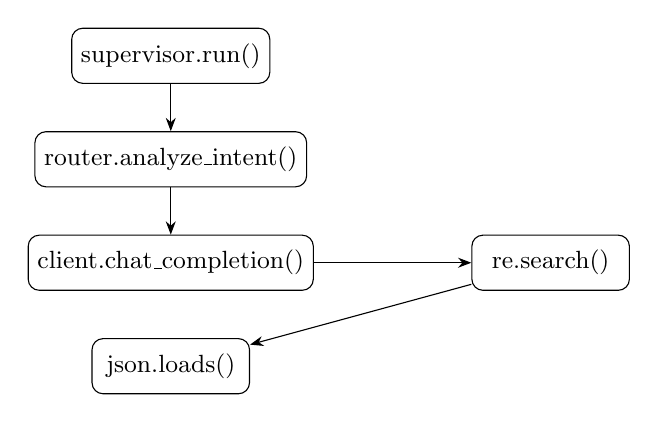
\begin{tikzpicture}[box/.style={draw, rounded corners, minimum width=2cm, minimum height=0.7cm, align=center, font=\small}, arrow/.style={->, >=Stealth}]
\node[box] (run) {supervisor.run()};
\node[box, below=0.6cm of run] (router) {router.analyze\_intent()};
\node[box, below=0.6cm of router] (llm) {client.chat\_completion()};
\node[box, right=2cm of llm] (re) {re.search()};
\node[box, below=0.6cm of llm] (json) {json.loads()};
\draw[arrow] (run) -- (router);
\draw[arrow] (router) -- (llm);
\draw[arrow] (llm) -- (re);
\draw[arrow] (re) -- (json);
\end{tikzpicture}
\end{center}

% ---------- 5.3 expert_sub_agents/base.py ----------
\section{expert\_sub\_agents/base.py —— 专家基类与自愈循环}

这是整个ACE Agent\textbf{最核心的创新点}——让AI写的代码自己修复自己。

\subsection{\_strip\_code\_fences() 辅助函数}

\begin{minted}{python}
def _strip_code_fences(text: str) -> str:
    """去除LLM经常在代码外包裹的markdown代码块标记"""
    if text is None:
        return ""
    stripped = text.strip()
    # 去掉开头的 ```python, ```py, 或 ```
    if stripped.startswith("```python"):
        stripped = stripped[len("```python"):]
    elif stripped.startswith("```py"):
        stripped = stripped[len("```py"):]
    elif stripped.startswith("```"):
        stripped = stripped[3:]
    # 去掉结尾的 ```
    if stripped.endswith("```"):
        stripped = stripped[:-3]
    return stripped.strip()
\end{minted}

\begin{plainbox}
    这个函数虽然简单但是关键——LLM经常返回\verb|```python\n你的代码\n```|，如果不去掉前后标记，沙箱中的\verb|exec()|会报SyntaxError。
\end{plainbox}

\subsection{BaseExpert.execute\_with\_self\_correction() —— 自愈循环核心}

这是整个项目\textbf{最值得深入理解}的方法。它体现了AI Agent的核心理念：\textbf{Think → Act → Fix}。

\begin{minted}[highlightlines={1-4,6-8,10-18,20-25}]{python}
def execute_with_self_correction(
    self, dataset: DatasetBundle, prompt: str, settings: LLMSettings
) -> list[AlgorithmRunResult]:
    # 第1步：Think —— LLM生成初始代码
    client = UniversalLLMClient(settings, caller=f"{self.key}:generate")
    results: list[AlgorithmRunResult] = []
    logs = [f"[{self.label}] 开始分析..."]

    raw_code = self._generate_code(client, dataset, prompt)  # 抽象方法，各专家自己实现
    code = _strip_code_fences(raw_code)                       # 清洗markdown标记

    # 第2步：Act + Fix 循环
    for attempt in range(1, self.MAX_RETRIES + 1):  # MAX_RETRIES = 3
        logs.append(f"[{self.label}] 第 {attempt} 次尝试运行代码...")
        try:
            run_result = self.sandbox.execute(code, dataset.X, dataset.y)
        except SandboxResourceExceeded as exc:
            # 资源超限直接终止，不重试
            logs.append(f"沙箱资源超限 ({exc.reason}): {exc.detail}")
            break

        # 第3步：判断结果，决定是继续循环还是退出
        if run_result["success"] and run_result["artifacts"]:
            # ✅ 完全成功：代码运行成功 + 有产出
            for algo, info in run_result["artifacts"].items():
                if algo.endswith("_error"):
                    continue  # 跳过错误占位条目
                # 构造 AlgorithmRunResult 加入结果列表
                results.append(AlgorithmRunResult(
                    algorithm_name=algo, expert_key=self.key,
                    expert_label=self.label, labels=info.get("labels"),
                    metrics=info.get("metrics", {}),
                    plot_path=Path(plot_raw) if plot_raw and Path(plot_raw).exists() else Path(""),
                    code=code,
                ))
            break  # 退出重试循环

        elif run_result["success"] and not run_result["artifacts"]:
            # ⚠️ 软失败：代码跑通了但没有按约定写入artifacts
            if attempt < self.MAX_RETRIES:
                # 构造专门的修复提示 → LLM重写代码
                diagnosis_hints = []
                if "if __name__" in code:
                    diagnosis_hints.append("- 删除 if __name__ == '__main__': 守卫")
                if "def main" in code or "def run" in code:
                    diagnosis_hints.append("- 不要用 def main(): 包裹逻辑")
                code = self._fix_code(fix_client, code, artifacts_hint, attempt=attempt)

        else:
            # ❌ 硬失败：代码运行时报错
            if attempt < self.MAX_RETRIES:
                # 将traceback发给LLM进行修复
                code = self._fix_code(fix_client, code, run_result["error"], attempt=attempt)
            else:
                logs.append("重试次数耗尽，任务失败。")
\end{minted}

\paragraph{三种结果状态的处理策略}

\begin{longtable}{p{3cm} p{3cm} p{7cm}}
    \toprule
    \textbf{状态} & \textbf{判定条件} & \textbf{处理策略} \\
    \midrule
    完全成功 & success=True \& artifacts非空 & 提取所有算法结果，退出循环 \\
    \midrule
    软失败 & success=True \& artifacts为空 & 分析常见原因（\_\_main\_\_守卫、未调用函数），注入诊断提示让LLM重写 \\
    \midrule
    硬失败 & success=False & 将完整traceback发给LLM，让LLM分析并修复代码 \\
    \midrule
    资源超限 & SandboxResourceExceeded & 直接终止，不重试（重试也无法解决OOM/超时） \\
    \bottomrule
\end{longtable}

\subsection{\_fix\_code() —— LLM驱动的代码修复}

\begin{minted}{python}
def _fix_code(self, client, old_code, error, *, attempt=1) -> str:
    system_prompt = (
        "你是一个 Python 调试专家。修正以下代码以解决给出的错误信息。"
        "只返回修正后的 Python 代码，不要解释。"
    )
    user_input = f"原始代码：\n{old_code}\n\n错误信息：\n{error}"
    reply = client.chat_completion(
        [{"role": "user", "content": user_input}], system_prompt,
        caller=f"{self.key}:fix:{attempt}", attempt=attempt,
    )
    return _strip_code_fences(reply or old_code)
\end{minted}

\begin{plainbox}
    这个方法就像一个"代码医生"——你把报错的代码和错误信息给它，它返回修复后的代码。如果LLM调用本身失败（reply为None），就返回原始代码（虽然可能仍然有问题，但至少不会丢代码）。
\end{plainbox}

\begin{tipbox}
    调试技巧：如果专家一直重试失败，检查 \texttt{self.last\_logs} 属性。每个BaseExpert实例在完成自愈循环后都会把每步日志存在 \texttt{last\_logs} 列表里。在测试中可以用 \texttt{expert.last\_logs} 查看完整的执行过程。
\end{tipbox}

% ---------- 5.3b expert_sub_agents/dimension_expert.py ----------
\section{expert\_sub\_agents/dimension\_expert.py —— 降维专家（Phase 3 混合模式）}

\textbf{Phase 3 架构亮点：} Dimension Expert 是 ACE Agent 中第一个采用"强类型骨架 + LLM 动态填空"混合模式的专家。与传统专家（LLM 生成完整 Python 代码 $\sim$4500 字符，错误率 $\sim$60\%）不同，Phase 3 将 LLM 从"代码生成器"降级为"参数决策器"。

\subsection{核心架构：骨架模板 + JSON 决策}

\begin{minted}{python}
# _SKELETON: 确定性 Python 骨架（~190 行）
# 1. 所有的 import / 异常守卫 / artifacts 写入已预写好
# 2. {DECISIONS_JSON} 占位符在运行时被 LLM JSON 决策替换

_SKELETON = r'''# ===== ACE Dimension Expert Skeleton (Phase 3) =====
import numpy as _np

_scaler = StandardScaler()          # 已由沙箱预注入
_X = _scaler.fit_transform(CTX_DATA.X)  # CTX_DATA 不可变数据上下文
_n = CTX_DATA.n_samples
_d = CTX_DATA.n_features
_k0 = CTX_DATA.expected_clusters

_DECISIONS = {DECISIONS_JSON}  # ← LLM 的 JSON 决策注入于此

# PIPELINE 1: PCA + KMeans
_d1 = _DECISIONS.get("pipelines", {}).get("pca_kmeans", {})
if _d1.get("active", True):
    ...  # 确定性的 PCA → KMeans → artifacts 写入
'''

# _generate_code() 调用流程:
# ① 构造用户消息（含 n_samples, n_features, expected_clusters, 维度类别）
# ② LLM 返回 ~140 token 的 JSON 决策（vs 旧方案 ~4500 字符代码）
# ③ JSON true/false/null → Python True/False/None 转换
# ④ 注入骨架 → 返回最终代码
\end{minted}

\subsection{5 条降维+聚类管线}

\begin{center}
\begin{tabular}{p{2.5cm} p{3cm} p{1.5cm} p{5.5cm}}
    \toprule
    \textbf{管线名} & \textbf{降维方法} & \textbf{聚类} & \textbf{激活条件} \\
    \midrule
    PCA\_KMeans  & PCA & KMeans & 几乎始终激活 \\
    PCA\_GMM     & PCA & GMM    & 几乎始终激活 \\
    UMAP\_KMeans & UMAP 流形学习 & KMeans & umap-learn 库可用时激活 \\
    tSNE\_KMeans & t-SNE 非线性降维 & KMeans & $n \leq 5000$ 自动限流 \\
    AE\_KMeans   & AutoEncoder 深度降维 & KMeans & $n\_features > 32$ 自动激活 \\
    \bottomrule
\end{tabular}
\end{center}

\subsection{沙箱预注入机制}

LLM 生成的代码\textbf{无需 import}任何 sklearn 核心模块。沙箱在代码执行前自动注入：

\begin{minted}{python}
# CORE_PRE_INJECT (coder_sandbox.py):
# StandardScaler, PCA, KMeans, GaussianMixture,
# silhouette_score, calinski_harabasz_score, davies_bouldin_score

# CTX_DATA (DataContext 不可变类):
# CTX_DATA.X, CTX_DATA.y, CTX_DATA.n_samples,
# CTX_DATA.n_features, CTX_DATA.expected_clusters
# 重新赋值 CTX_DATA.X = ... 会抛出 TypeError
\end{minted}

\subsection{Benchmark 实测数据（digits 64维）}

\begin{center}
\begin{tabular}{p{3cm} c c}
    \toprule
    \textbf{管线} & \textbf{ARI} & \textbf{Silhouette} \\
    \midrule
    PCA\_KMeans  & 0.4662 & 0.1591 \\
    PCA\_GMM     & 0.4484 & 0.1329 \\
    UMAP\_KMeans & \textbf{0.8764} & 0.1597 \\
    tSNE\_KMeans & 0.8491 & 0.1615 \\
    AE\_KMeans   & 0.3238 & 0.0710 \\
    \bottomrule
\end{tabular}
\end{center}

\textbf{关键指标：} Dimension Expert 16 轮运行 \textbf{100\% 成功率，零重试}（对比重构前 $\sim$60\% 成功率，平均 2.2 次重试）。UMAP\_KMeans 和 tSNE\_KMeans 两条管线包揽全局前两名。

\begin{tipbox}
    AE\_KMeans 当前分数偏低属预期行为：其使用浅层 MLP AutoEncoder（单隐层），在 64 维数据上容量有限。该管线的主要价值在 $>$128 维数据上才会充分体现；可通过增大 epochs (50–200) 或增加隐藏层深度来优化。
\end{tipbox}

% ---------- 5.4 agent_core/supervisor.py ----------
\section{agent\_core/supervisor.py —— 全局编排器}

\subsection{导入语句解释}

\begin{minted}{python}
from __future__ import annotations
import numpy as np
from datetime import datetime          # 标准库：生成带时间戳的输出目录名
from pathlib import Path                # 标准库：跨平台路径处理
from typing import Any, Dict, List, Optional

from ACE_Agent.agent_core.schemas import (  # 项目内数据模型
    SupervisorReport, DatasetBundle, RoutingDecision,
    AlgorithmRunResult, ProfileReport
)
from ACE_Agent.agent_core.router import MasterRouter       # 项目内：语义路由
from ACE_Agent.agent_brain.knowledge_engine import KnowledgeEngine  # 项目内：RAG
from ACE_Agent.expert_sub_agents import build_expert_registry        # 项目内：专家工厂
from ACE_Agent.tools.llm_client import UniversalLLMClient, LLMSettings
from ACE_Agent.tools.latex_generator import LatexReportGenerator
\end{minted}

\subsection{ACESupervisor类结构与关键设计}

\begin{minted}[highlightlines={1,3-6,8-10}]{python}
class ACESupervisor:
    """主控编排器 (Orchestrator)"""

    _DEFAULT_ACTIVE_EXPERTS: list[str] = ["centroid", "topology", "zoo", "critic"]

    def __init__(self) -> None:
        self.router = MasterRouter()                    # 创建路由
        self.knowledge_engine = KnowledgeEngine()       # 创建知识引擎
        try:
            self.knowledge_engine.ingest_docs()         # 注入知识库文档
        except Exception as e:
            print(f"知识库初始化警告: {e}")             # 非致命错误
        self.memory: list[dict[str, Any]] = []          # 会话记忆
        self.last_report: Optional[SupervisorReport] = None
        self.experts: dict[str, Any] = build_expert_registry()  # 专家注册表
\end{minted}

\textbf{第3行}：\verb|_DEFAULT_ACTIVE_EXPERTS| 是一个类属性（不是实例属性），意味着所有ACESupervisor实例共享这个默认列表。这种设计保证了默认行为的一致性。

\textbf{第8-10行}：知识库初始化用try/except包裹——即使知识库加载失败（比如ChromaDB模型未下载），系统仍可正常运行，只是RAG功能不可用。这体现了\textbf{优雅降级}的设计原则。

\subsection{run() 方法详解}

\begin{minted}[highlightlines={4-5,7-12,16-18,20-24}]{python}
def run(self, dataset, user_prompt, llm_settings, intent_data=None) -> SupervisorReport:
    # 1. 语义路由（若调用方已提前识别意图则跳过）
    if not intent_data:
        intent_data = self.router.analyze_intent(user_prompt, self.memory, llm_settings)
    intent = str(intent_data.get("intent", "NEW_TASK")).upper()

    # 2. RAG 增强
    knowledge_context = self.knowledge_engine.query(user_prompt)
    if knowledge_context:
        user_prompt = f"{knowledge_context}\n用户指令: {user_prompt}"

    # 3. 意图分流
    if intent == "FOLLOW_UP":
        return self._handle_follow_up(user_prompt, llm_settings, trace)
    if intent == "CODE_EXAMPLE":
        return self._handle_code_example(user_prompt, llm_settings, trace)

    # 4. NEW_TASK：必须有数据
    if not dataset:
        return self._error_report("未识别到数据。", trace, expert_logs={})

    # 5. 高维感知：自动激活维度专家
    n_features = dataset.X.shape[1]
    active_experts = list(self._DEFAULT_ACTIVE_EXPERTS)
    if n_features > 2 and "dimension" not in active_experts:
        trace.append(f"检测到数据维度为 {n_features}，已自动激活维度专家。")
        active_experts.append("dimension")

    return self._execute_full_analysis(dataset, user_prompt, llm_settings, trace, active_experts)
\end{minted}

\textbf{第4-5行}：\verb|intent_data| 参数允许调用方提前完成意图识别（比如Web UI可以先把用户输入分析完），避免重复调用LLM。这是一个\textbf{可选优化}。

\textbf{第7-12行}：RAG注入——如果知识库中有匹配的学术内容，直接拼到用户prompt前面。这样专家在生成代码时就能利用这些背景知识。

\textbf{第16-18行}：\verb|if not dataset|——这是安全网。如果意图是NEW\_TASK但没有数据集，不能继续（因为专家会尝试执行\verb|dataset.X.shape|而导致崩溃）。

\textbf{第20-24行}：高维感知——\verb|n_features > 2| 是阈值。2维数据可以直接可视化，但100维数据需要先降维才有意义。维度专家的自动激活体现了系统的\textbf{自适应能力}。

\subsection{\_execute\_full\_analysis() —— 并行专家执行}

\begin{minted}[highlightlines={5-15,17-20}]{python}
def _execute_full_analysis(self, dataset, prompt, settings, trace, active_experts):
    output_dir = self._prepare_output_dir(dataset.name)
    all_results: list[AlgorithmRunResult] = []
    expert_logs: dict[str, list[str]] = {}

    for key in active_experts:
        expert = self.experts.get(key)
        if expert is None:
            continue
        try:
            expert_results = expert.execute_with_self_correction(dataset, prompt, settings)
            all_results.extend(expert_results)
            expert_logs[key] = list(expert.last_logs)
        except Exception as exc:
            expert_logs[key] = [f"未捕获异常: {exc}"]

    if not all_results:
        return self._error_report("所有专家执行均失败。", trace, expert_logs=expert_logs)

    # 排序：按score降序
    ranking = sorted(all_results, key=lambda x: x.metrics.get("score", 0.0), reverse=True)

    # LLM生成摘要
    client = UniversalLLMClient(settings)
    best = ranking[0]
    summary = client.summarize_report({...})

    # 构造最终报告
    report = SupervisorReport(
        dataset=dataset, routing=RoutingDecision(...),
        results=all_results, ranking=ranking,
        executive_summary=summary or "聚类分析完成。",
        decision_trace=trace, response_type="CLUSTER_TASK",
    )
    # 自动生成LaTeX（静默失败）
    try:
        report.latex_path = LatexReportGenerator().generate(report)
    except Exception:
        pass

    self.last_report = report
    self.memory.append({"role": "user", "content": prompt})
    self.memory.append({"role": "assistant", "content": report.executive_summary})
    return report
\end{minted}

\textbf{第5-15行}：每个专家用try/except包裹——\textbf{一个专家失败不影响其他专家}。这是微服务架构的核心思想：隔离故障。

\textbf{第17-20行}：\verb|ranking = sorted(..., key=lambda x: x.metrics.get("score", 0.0), reverse=True)|——用lambda作为排序键，\verb|.get("score", 0.0)|确保即使某个算法的metrics中没有score字段也不会崩溃。

\begin{plainbox}
    说白了，Supervisor就像一个"项目经理"——它自己不干活，但负责把任务分给合适的人（专家），收集所有人的工作成果，汇总成一份总报告交给老板（用户）。
\end{plainbox}

\begin{notebox}
    易错点：如果在for循环中修改active\_experts列表（比如追加元素），可能导致迭代行为异常。这里用的是list(self.\_DEFAULT\_ACTIVE\_EXPERTS)浅拷贝，所以修改的是副本，不影响类属性。
\end{notebox}

% ---------- 5.5 tools/coder_sandbox.py ----------
\section{tools/coder\_sandbox.py —— 安全沙箱}

\subsection{安全策略设计}

\begin{minted}{python}
# 白名单：只允许这些内置函数在沙箱中可用
SAFE_BUILTINS: dict[str, Any] = {
    "__build_class__": __build_class__,  # 允许定义类
    "abs": abs, "all": all, "any": any,
    "dict": dict, "enumerate": enumerate,
    "float": float, "int": int, "len": len,
    "list": list, "max": max, "min": min,
    "print": print, "range": range,
    "round": round, "set": set, "str": str,
    "sum": sum, "tuple": tuple, "zip": zip,
    "Exception": Exception,  # 允许raise Exception
    # 注意：没有 open(), eval(), exec(), __import__() 等危险函数！
}
\end{minted}

\begin{plainbox}
    沙箱的安全策略是"白名单模式"——默认什么都不可用，只开放明确允许的。这比"黑名单模式"安全得多，因为黑名单总有漏网之鱼。
\end{plainbox}

\subsection{内存监控机制}

\begin{minted}{python}
class _MemoryWatchdog(threading.Thread):
    """后台线程每0.5秒检查一次内存增长量"""
    def __init__(self, limit_mb: int, poll_interval: float = 0.5):
        self.limit_mb = limit_mb
        self.exceeded = False
        # 记录基线：沙箱代码运行前的进程内存
        self._baseline_mb = psutil.Process(os.getpid()).memory_info().rss / (1024*1024)

    def run(self) -> None:
        while not self._stop_event.is_set():
            current_mb = proc.memory_info().rss / (1024 * 1024)
            delta_mb = max(0.0, current_mb - self._baseline_mb)  # 只计增量
            if delta_mb > self.limit_mb:
                self.exceeded = True  # 设置标志位
                return
            time.sleep(self.poll_interval)
\end{minted}

\textbf{关键设计}：监视的是内存\textbf{增量}（delta）而不是绝对值——这样不会把进程本身的基础内存（NumPy/PyTorch库等）计入限制。默认限制为2048MB（2GB），可通过环境变量\verb|ACE_SANDBOX_MEMORY_MB|调整。

\subsection{核心执行方法}

\begin{minted}[highlightlines={7-12,16,21-25}]{python}
def execute(self, code: str, X: np.ndarray, y=None) -> dict:
    artifacts: dict[str, Any] = {}              # ← 专家代码把结果写入这个字典
    exec_env: dict[str, Any] = {
        "__builtins__": SAFE_BUILTINS,          # ← 白名单内置函数
        "__name__": "__ace_sandbox__",          # ← 防止 __main__ 守卫
        "X": X,                                  # ← 数据直接注入
        "y": y,
        "artifacts": artifacts,                 # ← 结果字典
        "np": np,                                # ← 预导入numpy
    }

    # 配置Matplotlib（非交互式后端）
    try:
        matplotlib.use("Agg")
        import matplotlib.pyplot as plt
        if platform.system() == "Windows":
            plt.rcParams["font.sans-serif"] = ["Microsoft YaHei", "SimHei"]
        exec_env["plt"] = plt                   # ← 预配置的matplotlib
    except Exception:
        pass

    # 带资源限制执行
    self._run_with_limits(code, exec_env)

    # 救援逻辑：即使代码没写入artifacts，尝试从其他变量恢复
    if not artifacts:
        if "result" in exec_env and _looks_like_artifacts(exec_env["result"]):
            artifacts = exec_env["result"]  # 从旧版result变量恢复
        else:
            # 扫描所有用户自定义变量
            INJECTED = {"__builtins__", "__name__", "X", "y", "artifacts", "np", "plt"}
            for name, value in exec_env.items():
                if name not in INJECTED and _looks_like_artifacts(value):
                    artifacts = value
                    break
    return {"success": True, "artifacts": artifacts, "error": None}
\end{minted}

\textbf{第7-12行}：\verb|exec_env| 字典就是沙箱的"世界"。所有注入的变量（X, y, np, artifacts等）都在这个字典里，用户代码直接使用这些变量名即可。

\textbf{第16行}：\verb|__name__| 被设为 \verb|"__ace_sandbox__"|（不是 \verb|"__main__"|），这意味着如果LLM生成的代码中有 \verb|if __name__ == "__main__":| 守卫，里面的逻辑不会被执行。这就是为什么专家需要在软失败时检测并修复这种模式。

\textbf{第21-25行}：\textbf{救援逻辑（Rescue）}——这是P0.5阶段新增的功能。LLM有时会把结果写入名为\verb|result|或其他任意变量名，而不是约定的\verb|artifacts|。救援逻辑会扫描执行环境中的所有变量，找到"看起来像artifacts"的那个。

\subsection{\_looks\_like\_artifacts() 启发式检测}

\begin{minted}{python}
def _looks_like_artifacts(v: Any) -> bool:
    """检测一个变量是否"看起来像"artifacts字典"""
    if not isinstance(v, dict) or not v:
        return False
    for sub in v.values():
        if isinstance(sub, dict) and "labels" in sub:
            return True   # 找到了包含"labels"键的嵌套字典
    return False
\end{minted}

这个启发式函数检查变量的"形状"：必须是一个非空字典，且至少有一个值是包含"labels"键的字典。这样可以区分真正的算法结果字典和普通的配置字典（如\verb|{"seed": 42}|）。

\begin{tipbox}
    调试沙箱代码的最佳方式：在测试中直接调用 \texttt{sandbox.execute(code, X)}，检查返回的dict。如果success为False，error字段包含完整的traceback。也可以用 \texttt{exec(code, exec\_env)} 在本地调试（但要注意安全）。
\end{tipbox}

% ---------- 5.6 tools/llm_client.py ----------
\section{tools/llm\_client.py —— LLM客户端抽象层}

\subsection{架构设计：策略模式 + 门面模式}

\begin{center}
\begin{tikzpicture}[
    box/.style={draw, rounded corners, minimum width=2.8cm, minimum height=0.7cm,
                align=center, font=\footnotesize},
    arrow/.style={->, >=Stealth, thick},
    dasharrow/.style={->, >=Stealth, thick, dashed},
    node distance=0.8cm,
]
\node[box, fill=green!10] (client) {UniversalLLMClient\\(门面模式)};
\node[box, below left=0.5cm and -1.2cm of client, fill=yellow!5] (ds) {DeepSeekProvider};
\node[box, below=0.5cm of client, fill=yellow!5] (openai) {OpenAIProvider};
\node[box, below right=0.5cm and -1.2cm of client, fill=yellow!5] (ds2) {DashScopeProvider};
\node[box, below=0.8cm of openai, fill=blue!5] (abc) {LLMProvider (ABC)};
\draw[arrow] (client) -- (ds);
\draw[arrow] (client) -- (openai);
\draw[arrow] (client) -- (ds2);
\draw[dasharrow] (ds) |- (abc);
\draw[dasharrow] (openai) -- (abc);
\draw[dasharrow] (ds2) |- (abc);
\end{tikzpicture}
\end{center}

\begin{plainbox}
    UniversalLLMClient 相当于一个"万能遥控器"——不管你家电视是索尼还是三星（DeepSeek还是OpenAI），按同一个按钮（chat\_completion）都能工作。如果主电视坏了，自动切换到备用电视（回退机制）。
\end{plainbox}

\subsection{成本追踪与Trace记录}

每次LLM调用都会在\verb|outputs/llm_trace.jsonl|中追加一行JSON记录：

\begin{minted}{python}
trace_record = {
    "timestamp": "2026-04-25T10:30:00Z",
    "model": "deepseek-chat",
    "provider": "DeepSeek",
    "prompt_tokens": 1520,
    "completion_tokens": 380,
    "latency_ms": 2340,
    "caller": "centroid:generate",       # ← 标识谁调用的
    "is_retry": False,
    "attempt": 1,
    "fallback_triggered": False,
    "cost_usd": 0.000318                  # ← 估算费用
}
\end{minted}

这个设计让系统完全可观测——任何时候都可以通过读取trace文件了解：谁调用了LLM、花了多少token、多少钱、有没有回退。

\subsection{提供商回退机制}

\begin{minted}[highlightlines={3,5-6}]{python}
def chat_completion(self, messages, system_prompt=None, *, caller=None, attempt=1):
    try:
        reply = self._primary.chat(full_messages)      # 尝试主提供商
    except Exception as exc:
        # 判断是否需要回退
        status = self._http_status(exc)
        should_fallback = (
            self._fallback is not None
            and status in {429, 500, 502, 503, 504}    # ← 只在明确的服务端错误时回退
            or "timeout" in str(exc).lower()
        )
        if should_fallback:
            _write_trace({"event": "provider_fallback", "from_provider": ...})
            reply = self._fallback.chat(full_messages)  # ← 尝试备用提供商
\end{minted}

\textbf{第3行和第5-6行}：回退只在特定HTTP状态码（429/5xx）或超时时触发——如果是400类的客户端错误（如API key不对），回退到其他提供商也没用，不如直接报错。

% ---------- 5.7 tools/data_factory.py ----------
\section{tools/data\_factory.py —— 数据工厂}

\subsection{generate\_dataset() —— 数据集统一入口}

这个函数有约190行，我们重点讲解其设计模式：

\begin{minted}{python}
def generate_dataset(dataset_name: str, n_samples=480, noise=0.06, random_state=42):
    dataset_name = dataset_name.lower()

    if dataset_name == "blobs":
        X, y = make_blobs(n_samples=n_samples, centers=3, n_features=2, ...)
        return DatasetBundle(name="blobs", display_name="团状数据集", X=X,
                             shape_family="spherical", ...)

    if dataset_name == "moons":
        X, y = make_moons(n_samples=n_samples, noise=noise, ...)
        return DatasetBundle(name="moons", display_name="月牙数据集", X=X,
                             shape_family="non_convex", ...)
    # ... 更多数据集分支 ...
    raise ValueError(f"Unsupported dataset: {dataset_name}")
\end{minted}

\begin{plainbox}
    这个函数像一个"自动售货机"——你告诉它数据集的代号（如"moons"），它就返回一个包装好的DatasetBundle。内部使用scikit-learn的数据集生成器来创建数据。
\end{plainbox}

\subsection{load\_custom\_dataset() —— 自定义数据加载}

这个函数处理用户上传的CSV/Excel文件，包含几个重要设计：
\begin{enumerate}
    \item \textbf{自动类型转换}：遍历所有列，将object类型尝试转为数值
    \item \textbf{标签列自动检测}：最后一列如果唯一值很少（< 样本数的20\%），自动识别为标签列
    \item \textbf{缺失值处理}：用均值填充NaN值
    \item \textbf{数值列过滤}：只保留数值型特征列
\end{enumerate}

\begin{notebox}
    加载自定义CSV时常见问题：有些列全部是文字（如"姓名"列），load\_custom\_dataset()会跳过它们。但如果你想要的特征列被误判为文本（因为有特殊字符），需要预处理数据后再上传。
\end{notebox}

% ---------- 5.8 其余模块概览 ----------
\section{其余模块概览}

\subsection{expert\_sub\_agents/zoo\_expert.py —— 全量算法专家}

ZooExpert是唯一不调用LLM生成代码的专家。它的\verb|_generate_code()|使用\textbf{代码模板拼接}（code templating）的方式，直接构造包含10种算法的完整Python代码。这保证了算法逻辑的确定性——不像LLM生成代码那样可能有随机错误。

核心逻辑：
\begin{enumerate}
    \item 从AlgorithmZoo获取所有算法定义
    \item 为每个算法构造参数（将"expected\_clusters"占位符替换为实际值）
    \item 动态生成包含所有import、评估函数、绘图函数的完整代码
    \item 每个算法在try/except中独立运行，一个失败不影响其他
\end{enumerate}

\subsection{expert\_sub\_agents/critic\_expert.py —— 评价专家}

独立审计方，计算Hopkins统计量（聚类趋势指标）。\\[2pt]
H > 0.7：数据有明显的聚类趋势（适合聚类分析）。\\[2pt]
H $\approx$ 0.5：数据接近随机分布（聚类意义不大）。

\subsection{agent\_brain/knowledge\_engine.py —— 知识引擎}

使用ChromaDB向量数据库 + SentenceTransformer嵌入模型：
\begin{itemize}
    \item 扫描\verb|docs/|目录下的.md/.txt/.pdf文件
    \item 用滑动窗口（800字符窗口，200字符重叠）将文档分段
    \item 通过SentenceTransformer将每段转为768维向量存入ChromaDB
    \item 查询时用余弦相似度匹配最相关的3个片段
    \item 用manifest.json记录已入库文件，支持增量更新
\end{itemize}

\subsection{tools/latex\_generator.py —— LaTeX报告生成器}

将SupervisorReport转换为可编译的.tex文件：
\begin{itemize}
    \item 使用xeCJK宏包支持中文
    \item 转义所有LaTeX特殊字符（\_, \%, \$, etc.）
    \item CODE\_EXAMPLE类型的报告跳过生成（抛ValueError）
\end{itemize}

\subsection{web\_demo.py —— Streamlit Web界面}

约500行的Streamlit应用，提供：
\begin{itemize}
    \item 侧边栏：LLM配置、历史会话管理、成本监控面板
    \item 主区域：聊天式交互界面
    \item 数据集选择器：内置数据集或自定义上传
    \item 实时显示各专家的执行状态和结果图表
\end{itemize}

\begin{reviewbox}
    \begin{enumerate}
        \item 沙箱中为什么要把\verb|__name__|设为\verb|"__ace_sandbox__"|而不是\verb|"__main__"|？
        \item ZooExpert为什么不需要调用LLM？（提示：它与其他专家的核心区别是什么？）
        \item LLM客户端的回退机制在什么情况下不会触发？（提示：哪些HTTP状态码不会触发回退？）
    \end{enumerate}
\end{reviewbox}

% ============================================================================
% 第6章：数据存储与状态管理
% ============================================================================
\chapter{数据存储与状态管理}

\section{数据库/向量库结构}

ACE Agent 使用 ChromaDB（嵌入式向量数据库）存储学术参考文献：

\begin{center}
\begin{tikzpicture}[
    entity/.style={draw, rectangle, rounded corners, minimum width=3.5cm,
                   minimum height=0.9cm, align=center, font=\footnotesize},
    arrow/.style={->, >=Stealth, thick},
    node distance=0.9cm,
]
\node[entity, fill=blue!10] (col) {Collection: ace\_knowledge};
\node[entity, fill=green!5, below left=0.2cm and -2.0cm of col] (doc1)
     {文档1 (800字符块)\\id: taxonomy\_rules.md\_0};
\node[entity, fill=green!5, below=0.2cm of col] (doc2)
     {文档2 (800字符块)\\id: algorithm\_limits.md\_0};
\node[entity, fill=green!5, below right=0.2cm and -2.0cm of col] (doc3)
     {文档N (800字符块)\\id: paper.pdf\_5};
\draw[arrow] (col) -- (doc1);
\draw[arrow] (col) -- (doc2);
\draw[arrow] (col) -- (doc3);
\end{tikzpicture}
\end{center}

\paragraph{文档分段策略}
每个源文件被切成多个\textbf{重叠块}：
\begin{itemize}
    \item 块大小：800字符
    \item 重叠量：200字符（保证上下文连续性）
    \item 每个块转为768维向量（通过all-MiniLM-L6-v2模型）
\end{itemize}

\section{内存中的主要数据结构}

\subsection{会话记忆 (self.memory)}

\begin{minted}{python}
# 存储在 ACESupervisor.memory 中
self.memory = [
    {"role": "user", "content": "分析月牙数据集"},
    {"role": "assistant", "content": "聚类分析完成。最优算法为HDBSCAN..."},
    {"role": "user", "content": "为什么HDBSCAN比KMeans好？"},
    {"role": "assistant", "content": "因为月牙数据是非凸结构..."},
    # ... 更多对话轮次
]
\end{minted}

\subsection{专家执行日志 (expert\_logs)}

\begin{minted}{python}
# 存储在 _execute_full_analysis 方法的局部变量中
expert_logs = {
    "centroid": [
        "[质心专家] 开始分析数据特征并生成代码...",
        "[质心专家] 第 1 次尝试运行代码...",
        "[质心专家] 运行成功！",
    ],
    "topology": [
        "[拓扑专家] 开始分析数据特征并生成代码...",
        "[拓扑专家] 第 1 次尝试运行代码...",
        "[拓扑专家] 运行失败，错误信息: NameError: name 'NearestNeighbors' is not defined",
        "[拓扑专家] 正在分析错误并重写代码 (第1次重试)...",
        "[拓扑专家] 第 2 次尝试运行代码...",
        "[拓扑专家] 运行成功！",
    ],
    "zoo": [...],
    "critic": [...],
}
\end{minted}

\subsection{LLM追踪记录 (llm\_trace.jsonl)}

每行一个JSON对象，记录一次LLM调用的完整信息。Web界面的"LLM Call Monitor"面板通过读取这个文件来展示累计消耗。

\section{文件系统持久化}

\begin{longtable}{p{3.5cm} p{3cm} p{6.5cm}}
    \toprule
    \textbf{文件/目录} & \textbf{格式} & \textbf{内容} \\
    \midrule
    outputs/数据集名\_时间戳/ & 目录 & 每次分析的输出：raw\_data.png, 各算法聚类图, ace\_report.tex \\
    \midrule
    .ace\_demo\_config.json & JSON & LLM提供商选择、API keys、模型配置 \\
    \midrule
    .ace\_sessions.json & JSON数组 & 历史会话记录（对话历史 + 元数据） \\
    \midrule
    agent\_brain/memory\_vdb/ & ChromaDB & 知识库向量索引（SQLite3 + 向量数据） \\
    \midrule
    agent\_brain/ingested\_manifest.json & JSON数组 & 已入库文档清单（用于增量更新） \\
    \midrule
    outputs/llm\_trace.jsonl & JSONL & LLM调用追踪（每行一条记录） \\
    \bottomrule
\end{longtable}

\begin{reviewbox}
    \begin{enumerate}
        \item ChromaDB文档分段的窗口大小和重叠量是多少？为什么需要重叠？
        \item expert\_logs 在什么场景下被用于排错？（提示：看 \_error\_report 方法）
        \item .ace\_sessions.json 和 self.memory 的关系是什么？
    \end{enumerate}
\end{reviewbox}

% ============================================================================
% 第7章：完整运行示例
% ============================================================================
\chapter{完整运行示例（从启动到退出）}

本章模拟一次完整的ACE Agent使用过程，展示每一步的终端输出及背后发生的函数调用。

\section{Step 1：启动Web界面}

\begin{minted}{text}
$ streamlit run web_demo.py

  You can now view your Streamlit app in your browser.
  Local URL: http://localhost:8501
\end{minted}

\textbf{背后调用链}:
\begin{verbatim}
web_demo.py:main()
  → st.set_page_config()                     # 配置页面
  → _init_state()                            # 初始化session_state
    → _get_supervisor()                      # 创建ACESupervisor (带@st.cache_resource缓存)
      → ACESupervisor.__init__()
        → MasterRouter()                      # 创建路由
        → KnowledgeEngine()                   # 创建知识引擎
        → knowledge_engine.ingest_docs()       # 索引docs/目录
        → build_expert_registry()             # 创建所有专家实例
  → _sidebar_ui()                            # 渲染侧边栏
\end{verbatim}

\section{Step 2：配置LLM提供商}

用户点击"Model Config"，选择DeepSeek，输入API Key，点击保存。

\begin{minted}{text}
[UI] 显示 "保存配置" 按钮点击
\end{minted}

\textbf{背后调用链}:
\begin{verbatim}
SettingsStore.save({
    "active_provider": "DeepSeek",
    "api_keys": {"DeepSeek": "sk-xxx..."},
    "model": "deepseek-chat",
})
→ 写入 .ace_demo_config.json
→ st.rerun()  # 刷新页面
\end{verbatim}

\section{Step 3：执行聚类分析}

用户选择"月牙数据集"，输入\verb|"帮我分析这个数据集并推荐最佳算法"|。

\begin{minted}{text}
[ACE] 处理请求: 帮我分析这个数据集并推荐最佳算法
【主控】确认意图: NEW_TASK
【逻辑】用户明确要求分析数据集并推荐算法，属于新任务执行范畴
【RAG】成功检索到相关学术理论片段，已注入上下文。
【主控】检测到数据维度为 2，使用默认专家集。
\end{minted}

\textbf{背后调用链}:
\begin{verbatim}
supervisor.run(dataset=moons_bundle, user_prompt="帮我分析...", settings)
  → router.analyze_intent()                   # LLM判定 → NEW_TASK
  → knowledge_engine.query("帮我分析...")      # 检索相关理论
  → _execute_full_analysis(dataset, prompt, settings, trace, active_experts)
    → _prepare_output_dir("moons")            # 创建 outputs/moons_20260425_103000/
    → 并行执行:
      → centroid_expert.execute_with_self_correction()
        → _generate_code() → LLM返回KMeans/GMM代码
        → sandbox.execute(code, X, y)         # 第1次尝试即成功
        → 返回 [AlgorithmRunResult("KMeans", score=0.51, ...)]
      → topology_expert.execute_with_self_correction()
        → _generate_code() → LLM返回DBSCAN代码
        → sandbox.execute()                   # 第1次失败: NameError
        → _fix_code() → LLM修复代码
        → sandbox.execute()                   # 第2次成功
        → 返回 [AlgorithmRunResult("DBSCAN", score=0.92, ...)]
      → zoo_expert.execute_with_self_correction()
        → _generate_code() → 直接构造10种算法代码
        → sandbox.execute() → 10种算法串行运行
        → 返回 [AlgorithmRunResult*10]
      → critic_expert.execute_with_self_correction()
        → _generate_code() → LLM返回Hopkins代码
        → sandbox.execute()
        → 返回 [AlgorithmRunResult("Critic_Audit", ...)]
    → ranking = sorted(all_results, key=score, reverse=True)
    → LLM summarize_report() → 生成中文摘要
    → LatexReportGenerator.generate() → 生成ace_report.tex
    → 返回 SupervisorReport
\end{verbatim}

\section{Step 4：查看结果}

\begin{minted}{text}
[ACE 任务报告摘要]:
聚类分析完成！针对月牙数据集（200样本, 2特征），我们进行了多算法并行评估：

🏆 最优算法: DBSCAN (拓扑专家)
   - 综合得分: 0.920
   - 评分依据: Adjusted Rand Index (真实标签对比)
   - 关键优势: DBSCAN成功识别了月牙数据的非凸结构...

📊 算法排行榜:
  1. DBSCAN (拓扑专家) - score=0.920
  2. HDBSCAN (全量算法专家) - score=0.905
  3. SpectralClustering (全量算法专家) - score=0.873
  4. AgglomerativeClustering (全量算法专家) - score=0.761
  5. KMeans (质心专家) - score=0.512

💡 后续建议: 月牙数据集是典型的非凸数据集，基于密度的算法显著优于质心算法...
\end{minted}

\section{Step 5：追问}

用户继续输入\verb|"为什么HDBSCAN比DBSCAN在这个数据集上更好？"|。

\begin{minted}{text}
【主控】确认意图: FOLLOW_UP
【逻辑】用户在追问上一个分析结果的原因，属于FOLLOW_UP
【主控】正在基于知识库与会话上下文进行深度解析...

[ACE 分析回复]:
HDBSCAN 相比 DBSCAN 在这个数据集上的优势主要来自两点：
1. 自适应密度：HDBSCAN不需要设置全局密度阈值(eps)，...
2. 层次结构：HDBSCAN构建了密度层次树，...
\end{minted}

\textbf{背后调用链}:
\begin{verbatim}
supervisor.run(dataset=None, prompt="为什么HDBSCAN比DBSCAN...", settings)
  → router.analyze_intent()                   # LLM判定 → FOLLOW_UP
  → _handle_follow_up(prompt, settings, trace)
    → 获取 last_report 的摘要和排名作为上下文
    → LLM chat_completion() → 生成专业解释
    → 返回 SupervisorReport(response_type="FOLLOW_UP", ...)
\end{verbatim}

\section{关键变量演化追踪}

\begin{longtable}{p{2.5cm} p{2.5cm} p{8cm}}
    \toprule
    \textbf{变量} & \textbf{所属对象} & \textbf{演化过程} \\
    \midrule
    intent & supervisor.run()局部 & "NEW\_TASK" → 路由到完整分析流 \\
    \midrule
    active\_experts & supervisor.run()局部 & ["centroid", "topology", "zoo", "critic"]（2维数据，不激活dimension） \\
    \midrule
    all\_results & supervisor.\_execute\_full\_analysis()局部 & [] → 累积了约13个AlgorithmRunResult \\
    \midrule
    ranking & supervisor.\_execute\_full\_analysis()局部 & all\_results按score降序排列 \\
    \midrule
    self.last\_report & supervisor实例属性 & None → SupervisorReport（含所有结果） \\
    \midrule
    self.memory & supervisor实例属性 & [] → 追加了user和assistant两条记录 \\
    \bottomrule
\end{longtable}

\begin{reviewbox}
    \begin{enumerate}
        \item 为什么FOLLOW\_UP路径不需要传dataset？（提示：看\_handle\_follow\_up如何获取上下文）
        \item 在Step 3中，topology\_expert第1次执行为什么失败了？它通过什么机制修复？
        \item self.memory最多保留多少条历史记录？（提示：看analyze\_intent方法中history的使用方式）
    \end{enumerate}
\end{reviewbox}

% ============================================================================
% 第8章：扩展学习与常见坑
% ============================================================================
\chapter{扩展学习与常见坑}

\section{初学者最可能问的5个问题}

\subsection{Q1: 为什么代码要放在沙箱里执行，而不是直接在服务器上运行？}

\textbf{答}: LLM生成的代码是不可信的——它可能包含无限循环、恶意文件操作、或消耗大量内存导致服务器崩溃。沙箱通过以下机制防护：
\begin{itemize}
    \item 白名单内置函数（禁止open/eval/exec等）
    \item 60秒超时限制
    \item 2GB内存增长限制
    \item 隔离的命名空间（不影响主进程）
\end{itemize}
说白了，沙箱就像给AI写的代码戴上"手铐"，让它只能在一个受控的小房间里活动。

\subsection{Q2: BaseExpert的\_generate\_code()为什么是抽象方法？}

\textbf{答}: 因为每个专家有不同的"专业领域"——质心专家擅长KMeans，拓扑专家擅长DBSCAN。抽象方法强制每个子类必须实现自己的代码生成逻辑。这体现了\textbf{模板方法模式}：基类定义执行框架（自愈循环），子类填充具体逻辑（代码生成）。

\subsection{Q3: 为什么ZooExpert可以不调用LLM生成代码，其他专家要调用？}

\textbf{答}: ZooExpert使用\textbf{预置的代码模板}——10种算法的调用方式已经固化在\verb|AlgorithmZoo.get_algorithm_code()|中，不需要LLM"创作"。而其他专家需要根据用户的自然语言指令灵活调整代码（比如用户说"用KMeans比较不同k值的效果"），这需要LLM的理解能力。

\subsection{Q4: executor\_summary中的"score\_source"字段有什么意义？}

\textbf{答}: 不同评分标准有不同偏好：
\begin{itemize}
    \item \textbf{ARI}（Adjusted Rand Index）：需要真实标签，但对非凸簇形公正——DBSCAN在月牙数据上能得到高分
    \item \textbf{轮廓系数（Silhouette）}：不需要标签，但偏爱球形簇——KMeans得分会虚高
\end{itemize}
知道score\_source才能理解"为什么冠军算法赢了"——是因为它真的更好，还是因为评分标准对它有利？

\subsection{Q5: 整个项目的执行入口在哪里？}

\textbf{答}: 有两个入口：
\begin{itemize}
    \item \textbf{Web界面}: \verb|streamlit run web_demo.py| —— 适合交互式使用
    \item \textbf{命令行}: \verb|python demo_runner.py --dataset moons| —— 适合批处理/自动化
\end{itemize}
两者的核心逻辑都调用 \verb|ACESupervisor.run()|，只是UI层不同。

\section{3个改进方向（挑战练习）}

\subsection{练习1: 添加新的聚类算法}

\textbf{目标}: 在AlgorithmZoo中注册一个新算法（如BIRCH或MeanShift的替代方案）。

\textbf{步骤}:
\begin{enumerate}
    \item 在\verb|AlgorithmZoo.get_all_algorithms()|返回列表中添加新条目
    \item 确认ZooExpert的代码模板能处理新算法的调用方式
    \item 编写测试用例验证新算法在沙箱中正确执行
\end{enumerate}

\textbf{提示}: 检查\verb|_algo_map|字典是否需要扩展，以及fit/fit\_predict的使用方式。

\subsection{练习2: 实现真正的并行专家执行}

\textbf{目标}: 将Supervisor中顺序的for循环改为多线程/多进程并行。

\textbf{当前代码}（顺序执行）:
\begin{minted}{python}
for key in active_experts:
    expert = self.experts.get(key)
    expert_results = expert.execute_with_self_correction(...)
    all_results.extend(expert_results)
\end{minted}

\textbf{挑战}: 使用\verb|concurrent.futures.ThreadPoolExecutor|实现并行，并处理线程安全问题（Expert共享什么状态？需要加锁吗？）。

\subsection{练习3: 添加新的LLM提供商}

\textbf{目标}: 支持一个新的LLM API（如Claude/Gemini原生协议）。

\textbf{步骤}:
\begin{enumerate}
    \item 在\verb|llm_client.py|中创建继承\verb|OpenAICompatibleProvider|的子类
    \item 如果是非OpenAI兼容的API，需要重写\verb|chat()|方法
    \item 在\verb|_PROVIDER_CLASSES|字典中注册
    \item 在\verb|web_demo.py|的\verb|DEFAULT_PROVIDERS|和\verb|_COST_TABLE|中添加配置
\end{enumerate}

\section{常见调试场景}

\begin{tipbox}
    \textbf{场景1: 专家一直重试失败}\\
    检查 \texttt{expert.last\_logs} 看每步的日志。最常见的原因是LLM生成的代码缺少import或使用了沙箱禁用的内置函数。
\end{tipbox}

\begin{tipbox}
    \textbf{场景2: LLM返回的不是有效JSON}\\
    检查 \texttt{outputs/llm\_trace.jsonl} 看LLM实际返回了什么内容。Router用正则提取JSON，如果LLM返回格式变化，可能需要调整正则或system prompt。
\end{tipbox}

\begin{tipbox}
    \textbf{场景3: 沙箱超时}\\
    检查 \texttt{ACE\_SANDBOX\_TIMEOUT\_SEC} 环境变量。对于深度学习专家（DeepRepresentationExpert），默认60秒可能不够，可以调大。
\end{tipbox}

\begin{reviewbox}
    \begin{enumerate}
        \item 如果要添加一个"层次聚类专家"，需要在哪些文件中做修改？
        \item 为什么并行执行专家时需要注意线程安全？哪些共享状态可能存在竞态条件？
        \item 沙箱超时和内存超限的处理策略有什么不同？（提示：一个会重试，一个直接终止）
    \end{enumerate}
\end{reviewbox}

% ============================================================================
% 附录
% ============================================================================
\appendix
\chapter{环境配置速查}

\begin{minted}{text}
# 创建conda环境
conda create -n Tumor_Subtype_Agent python=3.10
conda activate Tumor_Subtype_Agent

# 安装依赖
pip install -r requirements.txt
pip install charset-normalizer  # 解决 Requests 依赖警告

# 配置LLM API Key
# 方式1: 环境变量
export ACE_DEEPSEEK_API_KEY="sk-your-key-here"
# 方式2: 在Web UI中配置（自动保存到 .ace_demo_config.json）

# 运行测试
pytest tests/ -v

# 启动Web界面
streamlit run web_demo.py

# 命令行运行
python demo_runner.py --dataset moons --interactive
\end{minted}

\chapter{术语表}

\begin{longtable}{p{3cm} p{10cm}}
    \toprule
    \textbf{术语} & \textbf{解释} \\
    \midrule
    LLM & 大语言模型（Large Language Model），如GPT-4、DeepSeek \\
    \midrule
    RAG & 检索增强生成（Retrieval-Augmented Generation）：在生成回答前先检索相关知识 \\
    \midrule
    自愈循环 & Think-Act-Fix循环：生成代码 → 执行 → 失败 → 分析错误 → 修复代码 → 重试 \\
    \midrule
    沙箱 & 受限制的执行环境，防止不受信任的代码造成损害 \\
    \midrule
    聚类 & 将数据点分成若干组（簇），使组内相似度高、组间相似度低 \\
    \midrule
    轮廓系数 & 一种聚类效果评估指标，范围[-1, 1]，越高越好 \\
    \midrule
    ARI & Adjusted Rand Index：调整兰德指数，衡量聚类结果与真实标签的一致性 \\
    \midrule
    Hopkins统计量 & 衡量数据聚类趋势的指标，>0.7表示明显趋势 \\
    \midrule
    PCA & 主成分分析：常用的线性降维方法 \\
    \midrule
    t-SNE & t分布随机邻域嵌入：非线性降维方法，适合可视化 \\
    \midrule
    DBSCAN & 基于密度的空间聚类算法，可发现任意形状的簇 \\
    \midrule
    HDBSCAN & DBSCAN的层次化改进版，自动适应不同密度区域 \\
    \midrule
    ChromaDB & 开源向量数据库，用于语义搜索 \\
    \midrule
    门面模式 & 设计模式：用一个统一接口封装多种底层实现 \\
    \midrule
    模板方法模式 & 设计模式：基类定义算法骨架，子类填充具体步骤 \\
    \bottomrule
\end{longtable}

\chapter{文件索引（按首字母排序）}

\begin{longtable}{p{5.5cm} p{7.5cm}}
    \toprule
    \textbf{文件路径} & \textbf{第章引用} \\
    \midrule
    agent\_brain/knowledge\_engine.py & 第5章第8节 \\
    \midrule
    agent\_core/router.py & 第5章第2节 \\
    \midrule
    agent\_core/schemas.py & 第5章第1节 \\
    \midrule
    agent\_core/supervisor.py & 第5章第4节 \\
    \midrule
    demo\_runner.py & 第7章 \\
    \midrule
    expert\_sub\_agents/base.py & 第5章第3节 \\
    \midrule
    expert\_sub\_agents/centroid\_expert.py & 第3章、第5章 \\
    \midrule
    expert\_sub\_agents/critic\_expert.py & 第5章第8节 \\
    \midrule
    expert\_sub\_agents/topology\_expert.py & 第3章、第5章 \\
    \midrule
    expert\_sub\_agents/zoo\_expert.py & 第5章第8节 \\
    \midrule
    tools/coder\_sandbox.py & 第5章第5节 \\
    \midrule
    tools/data\_factory.py & 第5章第7节 \\
    \midrule
    tools/latex\_generator.py & 第5章第8节 \\
    \midrule
    tools/llm\_client.py & 第5章第6节 \\
    \midrule
    tools/settings\_store.py & 第6章 \\
    \midrule
    web\_demo.py & 第5章第8节、第7章 \\
    \bottomrule
\end{longtable}

\end{document}
